\documentclass[a4paper,12pt]{article}
%%%%%%%%%%%%%%%%%%%%%%%%%%%%%%%%%%%%%%%%%%%%%%%%%%%%%%%%%%%%%%%%%%%%%%%%%%%%%%%%%%%%%%%%%%%%%%%%%%%%%%%%%%%%%%%%%%%%%%%%%%%%%%%%%%%%%%%%%%%%%%%%%%%%%%%%%%%%%%%%%%%%%%%%%%%%%%%%%%%%%%%%%%%%%%%%%%%%%%%%%%%%%%%%%%%%%%%%%%%%%%%%%%%%%%%%%%%%%%%%%%%%%%%%%%%%
\usepackage{eurosym}
\usepackage{vmargin}
\usepackage{amsmath}
\usepackage{fancyhdr}
%\usepackage{listings}
\usepackage{framed}
\usepackage{graphics}
\usepackage{epsfig}
\usepackage{subfigure}
\usepackage{fancyhdr}

\setcounter{MaxMatrixCols}{10}
%TCIDATA{OutputFilter=LATEX.DLL}
%TCIDATA{Version=5.00.0.2570}
%TCIDATA{<META NAME="SaveForMode" CONTENT="1">}
%TCIDATA{LastRevised=Wednesday, February 23, 2011 13:24:34}
%TCIDATA{<META NAME="GraphicsSave" CONTENT="32">}
%TCIDATA{Language=American English}

\pagestyle{fancy}
\setmarginsrb{20mm}{0mm}{20mm}{25mm}{12mm}{11mm}{0mm}{11mm}
\lhead{MA4704} \rhead{Mr. Kevin O'Brien}
\chead{Technological Mathematics 4}
%\input{tcilatex}

\begin{document}

\section*{Attempt 4 questions from 5}


\subsection*{Q.1 Descriptive Statistics (20 Marks)}
\subsubsection*{Part A} %28 MARKS
The table belwo presents the scores earned by 60 students in a statistics examination.
\begin{table}[ht]
\begin{center}
\begin{tabular}{|rrrrrrrrrr|}
\hline
42	&	43	&	44	&	44	&	45	&	45	&	46	&	47	&	51	&	52	\\
53	&	54	&	55	&	57	&	62	&	63	&	63	&	65	&	65	&	65	\\
66	&	66	&	69	&	71	&	72	&	72	&	73	&	74	&	74	&	75	\\
76	&	76	&	77	&	78	&	78	&	78	&	80	&	81	&	81	&	82	\\
82	&	82	&	83	&	84	&	84	&	85	&	85	&	86	&	87	&	88	\\
88	&	90	&	91	&	92	&	94	&	96	&	96	&	97	&	98	&	100	\\
\hline
\end{tabular}
\end{center}
\end{table}
\vspace{-0.5cm}
\begin{itemize}
\item[i.] (4 Marks) Summarize the data in the above table using a relative frequency table and a cumulative relative frequency table. Use 6 class intervals, with 41 as the lower limit of the first interval.
\item[ii.] (5 Marks) Draw a histogram for the above data. Comment on the shape of the histogram. Based on the shape of the histogram, what is the best measure of centrality and variability?
\item[iii.] (7 Marks) Construct a box plot for the above data. Clearly demonstrate how all of the necessary values were computed.
\end{itemize}

\vspace{0.25cm}
\subsubsection*{Part B} %10 MARKS
Data on the durations (measured in months) were collected for a random sample of product development projects.
The durations for these development projects were collected and tabulated as follows:

\begin{table}[ht]
\begin{center}
\begin{tabular}{|rrrrrrrr|}

\hline
12 & 11 & 20 & 19 & 18 & 9 & 16 & 15 \\
\hline
\end{tabular}
\end{center}
\end{table}
\vspace{-0.5cm}


\begin{itemize}
\item[i.](1 Mark) Calculate the mean of the project durations.
\item[ii.](2 Marks) Calculate the variance for this sample.
\item[iii.](1 Mark) Calculate the standard deviation for this sample.
\end{itemize}
%\item (2 marks) Calculate the coefficient of variation for country $A$.

%\item (2 marks) For the sample in country $B$, the mean of the durations was found to be 36 weeks, with a standard deviation of 6 weeks. In which country do the durations show a more dispersed distribution?


%A) Boxplot
%B) Histograms
%C) Mean, Median Variance etc

%----------------Boxplot
% 20 36 37 37 41 43 44 44 44 45
% 49 50 51 52 52 52 52 53 53 53
% 54 55 55 57 57 59 59 59 62 62
% 65 66 67 70 71 74 86 87 89 98

%Outliers : 20,  89, 98
%Fences :  22.25 , 88.25
%

%------------------------------------------------------------------------------------------------ %
\newpage
\subsection*{Q.2 Probability (20 Marks)}
\subsubsection*{Part A}
Competitors A and B fire at their respective targets. The probability that A hits a target is 1/3 and the probability that B hits a target is 1/5. Find the probability that:
\begin{itemize}
\item[i.] (2 marks) A does not hit the target,
\item[ii.](2 marks)  both hit their respective targets,
\item[iii.](2 marks)  only one of them hits a target,
\item[iv.](2 marks) neither A nor B hit their targets.
\end{itemize}

\subsubsection*{Part B}
On completion of a programming project, three programmers from a team submit a collection of subroutines to an acceptance group. \\
    \\
    The following table shows the percentage of subroutines each programmer submitted and the probability that a subroutine submitted by each programmer will pass the certification test based on historical data.

\begin{center}
\begin{tabular}{|l|c|c|c|}
  \hline
Programmer &	A	&B	& C	\\\hline
Proportion of subroutines submitted&	0.40	&0.35	&0.25	\\ \hline
Probability of acceptance	&0.75	&0.95	&0.85\\

  \hline
\end{tabular}
\end{center}

\begin{itemize}
\item[i.] (3 marks) What is the proportion of subroutines that pass the acceptance test?
\item[ii.](3 marks)  After the acceptance tests are completed, one of the subroutines is selected at random and found to have passed the test. What is the probability that it was written by Programmer A?
\end{itemize}


%Question 2
%A) Expected Values
%b) Probability
%C) Bayes Theorem
%D) Testing Normality +  p.value questions
\subsubsection*{Part C}
 The probability distribution of discrete random variable $X$ is tabulated below. There are 6 possible outcome of $X$, i.e. 0, 1, 2, 4 ,8 and 10.
\begin{center}
\begin{tabular}{|c||c|c|c|c|c|c|}
\hline
$x_i$  & 0 & 1 & 2 & 4 & 8 & 10 \\\hline
$P(x_i)$ & 0.25 & 0.15 & 0.25 & 0.15 & k & 0.10\\
\hline
\end{tabular}
\end{center}

\begin{itemize}
\item[i.] (1 marks) Compute the value for $k$.
\item[ii.] (3 marks) Determine the expected value $E(X)$.
\item[iii.] (2 marks) Evaluate $E(X^2)$.
%\item[iv.] (3 marks) Compute the variance of random variable $X$.
\end{itemize}



%------------------------------------------------------------------------------------------------ %
\newpage
%Question 3
%A) Normal Distribution 8 Marks
%B) Binomial Distribution - Not Actioned
%C) Poisson 6 Marks
%D) Exponential 6 Marks

% Almost Ready

\subsection*{Q.3 Probability Distributions (20 Marks)}

\subsubsection*{Part A} % Exponential %6 MARKS
Suppose that a student is taking a multiple-choice exam in which each question has four possible answers to choose from. There are ten questions in the exam.
Suppose that she has no knowledge of the correct answer to any of the questions. Furthermore, suppose that she selects one of the possible choices at random as her answer.

\begin{itemize}
\item[i.] (2 marks)	What is the probability that she will answer four questions correctly.
\item[ii.] (2 marks) What is the probability that she will get at least three correct answers?
\item[iii.] (2 marks) What is the probability that she will answer none of the questions correctly?
%\item[iv.] (2 marks) What is the probability that she will answer at least one question correctly?
\end{itemize}

\subsubsection*{Part B}% Poisson %6 MARKS
Telephone calls arrive at a switchboard at a rate of 45 per hour. Calculate the following:

\begin{itemize}
\item [i.](2 Marks)	The probability of 3 or more calls arriving in any 4 minute period,
\item [ii.](2 Marks) The probability of no phone calls arriving in a 4 minute period,
\item [iii.](2 Marks) The probability of exactly five phone call arriving in a 12 minute period.
%\item [iv.]	The average and standard deviation of the number of phone calls arriving in a 2 minute period.

\end{itemize}
\subsubsection*{Part C} %NORMAL %8 MARKS
Assume that the length of injected moulded plastic components are normally distributed with a mean of 12.5mm and a standard deviation of 2.5mm.  Calculate the corresponding probability for the following measurements occurring on an individual component.

\begin{itemize}
\item [i.](2 Marks)	Between 12.5 and 15mms,
\item [ii.](2 Marks) Less than 10 mms,
\item [iii.](2 Marks) Between 12 and 15 mms,
\item [iv.](2 Marks) Less than 10.3 mms.
\end{itemize}
\noindent Illustrate each of your answers with a sketch.
%------------------------------------------------------------------------------------------------ %
\newpage

% Question 4  Hypothesis Testing  + Confidence Intervals
% Good Shape

\subsection*{Q4. Inference Procedures (20 Marks)}

\subsubsection*{Part A} %4 Marks
\begin{itemize}
\item[i.](2 Marks) In the context of hypothesis testing, explain what a p-value is, and how it is used. Support your answer with a simple example.
\item[ii.](2 Marks) What is meant by Type I error and Type II error?
\end{itemize}
\subsubsection*{Part B} %3 Marks
A well-known polling company estimates that $57\%$ of Irish voters support a new constitutional amendment. 800 people were randomly surveyed and asked about their voting preferences. 482 of the 800 people responded positively to the amendment. You are required to:

\begin{itemize}
\item [i.](2 Marks) Construct a 95\% confidence interval for the proportion of people in favour of the constitutional amendment.
\item[ii.] (2 Marks) Based on this confidence interval, what is your conclusion regaring the estimate made by the polling company. Justify your answer.
\end{itemize}

\subsubsection*{Part C} %4 Marks
 The data set \texttt{X} and \texttt{Y} are both assumed to be normally distributed. The Shapiro-Wilk test was carried out to assess whether or not this assumption is valid for data set \texttt{X}.
\begin{itemize}
\item[i.] (1 marks) Formally state the null and alternative hypothesis.
\item[ii.] (2 marks) What is your conclusion for this procedure? Justify your answer.
\end{itemize}
\begin{framed}
\begin{verbatim}
> shapiro.test(X)

        Shapiro-Wilk normality test

data:  X
W = 0.9292, p-value = 0.372
\end{verbatim}
\end{framed}
\bigskip
\newpage
\subsubsection*{Part D}
The data set \texttt{X} and \texttt{Y} are both assumed to be normally distributed. A graphical procedure was carried out to assess whether or not this assumption of normality is valid for data set \texttt{Y}. Consider the Q-Q plot in the figure below.

\begin{center}
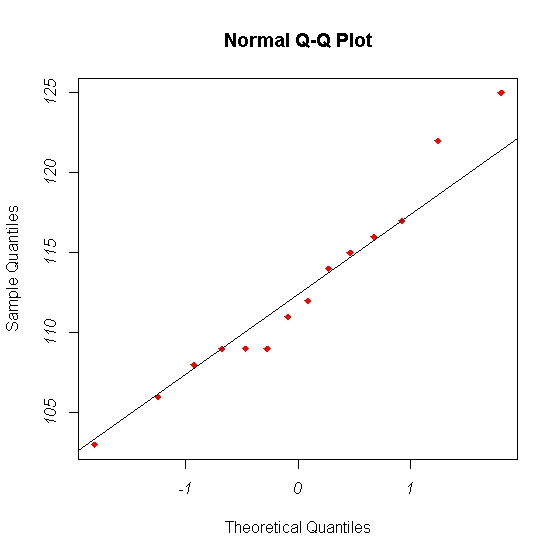
\includegraphics[scale=0.55]{Q5examQQplot}
\end{center}

\begin{itemize}
\item[i.] (2 marks) Provide a brief description on how to interpret this plot.
\item[ii.] (1 marks) What is your conclusion for this procedure? Justify your answer.
\end{itemize}

\subsubsection*{Part E} %9 Marks
The operating life span of a new electronic component produced by Echelon is assumed to be approximately normally distributed.\\\\
    A sample of 80 components was tested by Echelon's design department. The key findings of this study are as follows: the mean life span for the sample components was found to be 8950 hours, with standard deviation of 600 hours.\\\\ Echelon designed the component to have a mean life span of 8800 hours. Perform an appropriate significance test for the hypothesis that this specification was met.


\begin{itemize}
\item[i.] (2 marks) Clearly state the null and alternative hypothesis for this procedure.
\item[ii.] (2 marks) Compute the appropriate test statistic.
\item[iii.] (2 marks) What is your conclusion for this procedure? Justify your answer.
%\item[iv.] (2 marks) Provide a $95\%$ confidence interval for the population mean.
\end{itemize}

%Calculate a 95\% confidence interval for the difference between the mean number of marks obtained by males and females in the population of school leavers as a whole.
%(7 marks)


% State your hypotheses clearly. What is the significance level of this test?
\bigskip

%        1-sample proportions test with continuity correction
%
% data:  482 out of 800, null probability 0.57
% X-squared = 3.3162, df = 1, p-value = 0.0686
% alternative hypothesis: true p is not equal to 0.57
% 95 percent confidence interval:
% 0.5675450 0.6364573
% sample estimates:
%     p
% 0.6025

%-------------------------------------------------------------------------------------------------- %
\newpage
\subsection*{Q5. Correlation and Linear Regression (20 Marks)} %NOT READY
% Correlation and Simple Linear Regression
% Non Parametric Procedures

A wood scientist wanted to establish if there was a relationship between the adhesive strength of laminated wood and the dwell time in press machine. A random sample of 9 different times and their corresponding adhesive strengths in pounds per square inch (PSI) were recorded as follows:

\begin{center}
\begin{tabular}{|c|c|c|}

  \hline
Sample &Time (Mins) & Pull Strength (PSI) \\
 & (X)  &  (Y)\\ \hline
1& 5.0& 3.5 \\
2& 4.8& 3.3\\
3& 5.6& 3.9\\
4& 4.3& 2.7\\
5& 4.2& 3.2\\
6& 5.4& 4.1\\
7& 5.5& 4.3\\
8& 4.0& 2.8\\
9& 4.7& 3.7\\
  \hline
\end{tabular}
\bigskip

\begin{tabular}{lll}
  $\sum X = 43.5$ & $\sum Y = 31.5$ & $\sum XY = 154.61$ \\
  $\sum X^2 = 213.03$ & $\sum Y^2 = 112.71$ &  \\
 \end{tabular}
 \end{center}
%> sum(X)
%[1] 43.5
%> sum(Y)
%[1] 31.5
%> sum(X*Y)
%[1] 154.61
%> sum(X^2)
%[1] 213.03
%> sum(Y^2)
%[1] 112.71

\begin{itemize}
\item[i.](5 Marks) Draw a scatter-plot and comment on its features.
\item[ii.](5 Marks) Calculate the correlation coefficient. Interpret your answer.
\item[iii.](5 Marks) Calculate the equation of the least squares regression line and interpret the value of the slope.
\item[iv.](3 Marks) Using this regression model, estimate the adhesive strength for a piece of wood that has been in the press machine for 7 minutes.
\item[v.](2 Marks) Is such an estimate reliable? Briefly explain why.
\end{itemize}



%-------------------------------------------------------------------------------------------------- % \newpage
\newpage
\section*{Formulae}
%-------------------------------------------------%
\subsection*{Descriptive Statistics}
\begin{itemize}
\item Sample Variance
\begin{equation*}
s^2 = \frac{\sum (x-\bar{x})^2}{n-1}
\end{equation*}
\end{itemize}
%-------------------------------------------------%
\subsection*{Probability}
\begin{itemize}

\item Conditional probability:
\begin{equation*}
P(B|A)=\frac{P\left( A\text{ and }B\right) }{P\left( A\right) }.
\end{equation*}


\item Bayes' Theorem:
\begin{equation*}
P(B|A)=\frac{P\left(A|B\right) \times P(B) }{P\left( A\right) }.
\end{equation*}





\item Binomial probability distribution:
\begin{equation*}
P(X = k) = ^{n}C_{k} \times p^{k} \times \left( 1-p\right) ^{n-k}\qquad \left( \text{where  }
^{n}C_{k} =\frac{n!}{k!\left(n-k\right) !}. \right)
\end{equation*}

\item Poisson probability distribution:
\begin{equation*}
P(X = k) =\frac{m^{k}\mathrm{e}^{-m}}{k!}.
\end{equation*}

\item Exponential probability distribution:
\begin{equation*}
P(X \leq k) = \begin{cases}
1-e^{- k/\mu}, & k \ge 0, \\
0, & k < 0.
\end{cases}\qquad \left( \text{where  }
\mu = {1\over \lambda}\right)
\end{equation*}
\end{itemize}



\subsection*{Confidence Intervals}
{\bf One sample}
\begin{eqnarray*} S.E.(\bar{X})&=&\frac{\sigma}{\sqrt{n}}.\\\\
S.E.(\hat{P})&=&\sqrt{\frac{\hat{p}\times(100-\hat{p})}{n}}.\\
\end{eqnarray*}
{\bf Two samples}
\begin{eqnarray*}
S.E.(\bar{X}_1-\bar{X}_2)&=&\sqrt{\frac{\sigma^2_1}{n_1}+\frac{\sigma_2^2}{n_2}}.\\\\
S.E.(\hat{P_1}-\hat{P_2})&=&\sqrt{\frac{\hat{p}_1\times(100-\hat{p}_1)}{n_1}+\frac{\hat{p}_2\times(100-\hat{p}_2)}{n_2}}.\\\\
\end{eqnarray*}
\subsection*{Hypothesis tests}
{\bf One sample}
\begin{eqnarray*}
S.E.(\bar{X})&=&\frac{\sigma}{\sqrt{n}}.\\\\
S.E.(\pi)&=&\sqrt{\frac{\pi\times(100-\pi)}{n}}
\end{eqnarray*}
{\bf Two large independent samples}
\begin{eqnarray*}
S.E.(\bar{X}_1-\bar{X}_2)&=&\sqrt{\frac{\sigma^2_1}{n_1}+\frac{\sigma_2^2}{n_2}}.\\\\
S.E.(\hat{P_1}-\hat{P_2})&=&\sqrt{\left(\bar{p}\times(100-\bar{p})\right)\left(\frac{1}{n_1}+\frac{1}{n_2}\right)}.\\
\end{eqnarray*}
{\bf Two small independent samples}
\begin{eqnarray*}
S.E.(\bar{X}_1-\bar{X}_2)&=&\sqrt{s_p^2\left(\frac{1}{n_1}+\frac{1}{n_2}\right)}.\\\\
s_p^2&=&\frac{s_1^2(n_1-1)+s_2^2(n_2-1)}{n_1+n_2-2}.\\
\end{eqnarray*}
{\bf Paired sample}
\begin{eqnarray*}
S.E.(\bar{d})&=&\frac{s_d}{\sqrt{n}}.\\\\
\end{eqnarray*}
{\bf Standard Deviation of case-wise differences (computational formula)}
\begin{eqnarray*}
s_d = \sqrt{ {\sum d_i^2 - n\bar{d}^2 \over n-1}}.\\\\
\end{eqnarray*}


\noindent{\bf Regression estimates}

\begin{eqnarray*}
S_{XY} &=&
\sum x_iy_i - \frac{\sum x_i\sum y_i}{n}\\
S_{XX} &=&
\sum x_i^2 - \frac{(\sum x_i)^2}{n}\\
S_{YY} &=&
\sum y_i^2 - \frac{(\sum y_i)^2}{n}\\
\end{eqnarray*}
{\bf Slope Estimate}
\begin{eqnarray*}
b_1 = \frac{S_{XY}}{S_{XX}}
\end{eqnarray*}
{\bf Intercept Estimate}
\begin{eqnarray*}
 b_0 = \bar{y} -b_1\bar{x}
\end{eqnarray*}
{\bf Pearson's correlation coefficient}

\begin{eqnarray*}
r = \frac{S_{XY}}{\sqrt{S_{XX} \times S_{YY}}}
\end{eqnarray*}
{\bf Standard error of the Slope}
\begin{eqnarray*}
S.E.(b1) = \sqrt{\frac{s^2}{S_{XX}}}
\end{eqnarray*}

where $s^2 = \frac{SSE}{n-2}$
and SSE $= S_{YY} - b_1S_{XY}$
\end{document} 